\documentclass[a4paper]{article}

% Enables the inclusion of images using
% the \includegraphics directive
\usepackage{graphicx}

% Allows forceful placement of figures
% using the [H] option for figures.
\usepackage{float}

\usepackage{booktabs}

% Replace paragraph-indents with linebreaks between paragraphs
\usepackage{parskip}
\usepackage{minted}
\usepackage{amsmath}

\usepackage{algorithm}
\usepackage[noend]{algpseudocode}

% Allows us to define our own macros
\usepackage{letltxmacro}
\LetLtxMacro\tt\texttt
\LetLtxMacro\mi\mintinline

\newcommand{\opcode}{Opcode\ }
\newcommand{\format}{Format\ }
\newcommand{\integer}{Integer32\ }
\newcommand{\opcodem}{\mintinline{java}{Opcode}\ }
\newcommand{\formatm}{\mintinline{java}{Format}\ }
\newcommand{\instructionm}{\mintinline{java}{Instruction}\ }
\newcommand{\decomposedm}{\mintinline{java}{DecomposedRepresentation}\ }
\newcommand{\mnemonicm}{\mintinline{java}{MnemonicRepresentation}\ }
\newcommand{\registerm}{\mintinline{java}{Register}\ }
\newcommand{\mij}[1]{\mintinline{java}{#1}}

\usepackage{xcolor}
\definecolor{mintedbackground}{rgb}{0.95,0.95,0.95}

\begin{document}

\section{Introduction}

In the MIPS32 architecture, all machine instructions are represented
as 32-bit numbers. This article presents a MIPS32-decompiler that,
when passed 32-bit numbers which either partially or completely
represent MIPS32 instructions yields a series of different
representations of the same instruction.

Specifically, MIPS32 instructions are to be read from a file with
numbers either in decimal or hexadecimal form. For each number in the
input file, the disassembler will produce the following:

\begin{itemize}
  \item The number from the input file.
  \item The format of the instruction (R, I, or J).
  \item The decomposed representation in decimal.
  \item The decomposed representation in hexadecimal.
  \item The representation of the instruction in mnemonic format,
    using register abbreviations wherever possible (e.g.,
    \texttt{\$t0} instead of \texttt{\$8}) and using decimal numbers
    whenever actual numbers are necessary.
\end{itemize}

In the following subsections an introduction of the terminology used
throughout this document is provided. Afterwards you may refer to this
section again if any of the above requirements seem foreign to you.

The rest of the document will be dedicated to a high-level description
of this solution accompanied with a guide on how to compile and run
the software.

The appendix contains an overview of all those instructions that the
decompiler is capable of comprehending.

\subsection{Terminology}

% TODO: cite
According to Aho et al.  a \emph{compiler} is a program that
can read a program in one language --- the \emph{source} language --
and translates it into an equivalent program in another language --
the \emph{target} language; see Fig. \ref{fig:compiler}.

\begin{figure}[H]
  \centering
  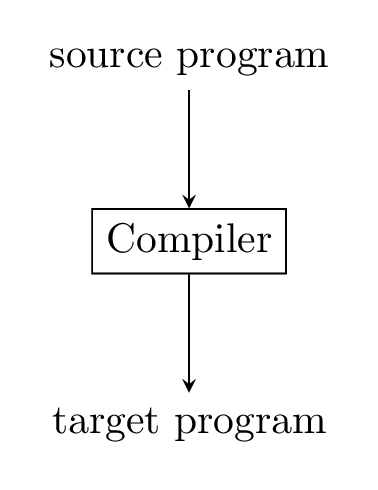
\includegraphics[width=0.3\textwidth]{figures/compiler.png}
  \caption{A compiler}
  \label{fig:compiler}
\end{figure}

Conversely, a \emph{decompiler} is also a that performs the reverse
operation of a compiler. It too, is a compiler. Commonly one views a
compiler as a translator from a high-level human-readable source
language into a low-level machine-readable language, similarly a
decompiler translates in the opposite direction; see
Fig. \ref{fig:decompiler}. 

The two exhibit a chiral relation to one another, i. e. that they are
mirrored images of each other in terms of functionality, but they are
not themselves identical.

\begin{figure}[H]
  \centering
  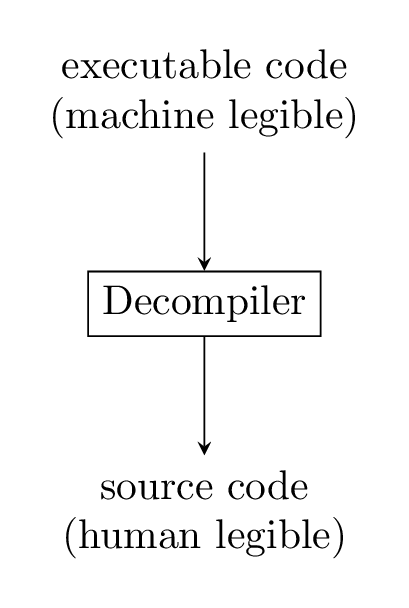
\includegraphics[width=0.3\textwidth]{figures/decompiler.png}
  \caption{A decompiler}
  \label{fig:decompiler}
\end{figure}

\subsection{Key concepts}

In this assignment the decompiler must be able to translate from the
machine-readable language of 32-bit numbers representing MIPS32
instructions to the human-readable target language described in the
introduction.

By example, the constituent parts of the decompilers output will
be described further.

Specifically,

\begin{itemize}
  \item Format.
  \item Opcode.
  \item Decomposed representation.
  \item Mnemonic representation.
\end{itemize}

will be covered. We will augment this list later on.

\subsubsection{Example: Decomposing \texttt{mul}}

Consider the 32-bit number \texttt{0x71014802}. It is \emph{decomposed}
into fields of varying lengths depending on the \emph{format} of the
instruction.

For all numbers in the MIPS32 instruction set the leftmost six bits
always represent the opcode for the instruction. The opcode alone is
not always sufficient to identify the particular instruction,
\emph{but} it is always sufficient to identify the format of the
instruction.

The leftmost six bits of \texttt{0x71014802} is \texttt{0x1c}. It is
\emph{known} that this number corresponds to an instruction in the
R-format. The format specifies into which fields the remaining bits
decompose into. In Fig. \ref{fig:r-decomposed} each field's size in
bits is the small number below the field.

\begin{figure}[H]
  \centering
  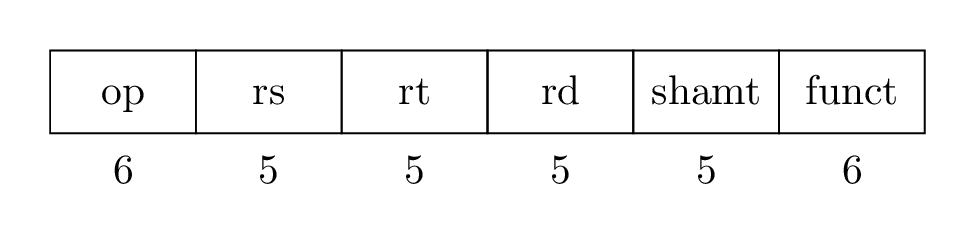
\includegraphics[width=0.9\textwidth]{figures/r-decomposed.png}
  \caption{The fields of an R-type instruction}
  \label{fig:r-decomposed}
\end{figure}

As alluded to previously, all instructions may not be discerned by
their opcode alone. This holds for all R-type instructions.

Decomposing \texttt{0x71014802} into the fields shown in
Fig. \ref{fig:r-decomposed} yields \texttt{rs=8}, \texttt{rt=1},
\texttt{rd=9}, \texttt{shamt=0}, and \texttt{funct=2}. The
\emph{decomposed representation} of this instruction in hexadecimal
form is thus \texttt{[0x1c 8 1 9 0 2]}.\footnote{The corresponding
\emph{decimal representation} is \texttt{[28 8 1 9 0 2]}}

To identify the particular instruction represented by
\texttt{0x71014802} the \texttt{funct} field must be
consulted. Pairing the opcode, \texttt{0x1c} and the value in the
\texttt{funct} field uniquely identifies the instruction a
\texttt{mul} instruction; see Fig. \ref{fig:mul-decomposed}

\begin{figure}[H]
  \centering
  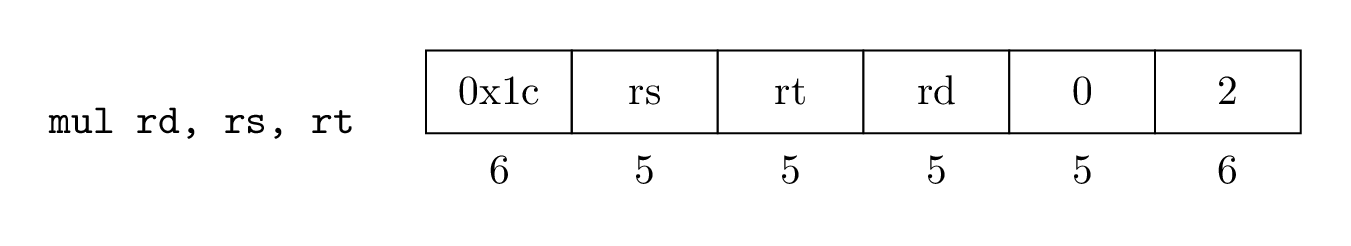
\includegraphics[width=0.9\textwidth]{figures/mul-decomposed.png}
  \caption{Decomposition and mnemonic representation of \texttt{mul}}
  \label{fig:mul-decomposed}
\end{figure}

From Fig. \ref{fig:r-decomposed} the registers \texttt{rs},
\texttt{rt} and \texttt{rd} were determined to have the addresses 8,
1, and 9, respectively. In MIPS registers are named, following the
convention shown in Table. \ref{table:mips-register-naming-convention}

\begin{table}[H]
\centering
\caption{MIPS register naming convention}
\begin{tabular}{ll}
\toprule
Nickname & Register Number \\
\midrule
\$zero      & 0            \\
\$at        & 1            \\
\$v0 - \$v1 & 2 - 3        \\
\$a0 - \$a3 & 4 - 7        \\
\$t0 - \$t7 & 8 - 15       \\
\$s0 - \$s7 & 16 - 23      \\
\$t8 - \$t9 & 24 - 25      \\
\$k0 - \$k1 & 26 - 27      \\
\$gp        & 28           \\
\$sp        & 29           \\
\$fp        & 30           \\
\$rd        & 31           \\
\bottomrule
\end{tabular}
\label{table:mips-register-naming-convention}
\end{table}

Replacing the numerical values of \texttt{rs}, \texttt{rt} and
\texttt{rd}, with their named counterparts yields the \emph{mnemonic
representation} of the instruction to be

\begin{center}
  \texttt{mul \$t1, \$t0, \$at}
\end{center}

\subsection{Problem statement}

In this assignment the core functionality which is exposed is
\emph{parsing} such a 32-bit number representing an instruction from
the MIPS32-instruction set and outputting other representations of the
same instruction, as well as some additional information regarding the
very same instruction, see Fig. \ref{fig:mips32-decompiler}.

\begin{figure}[H]
  \centering
  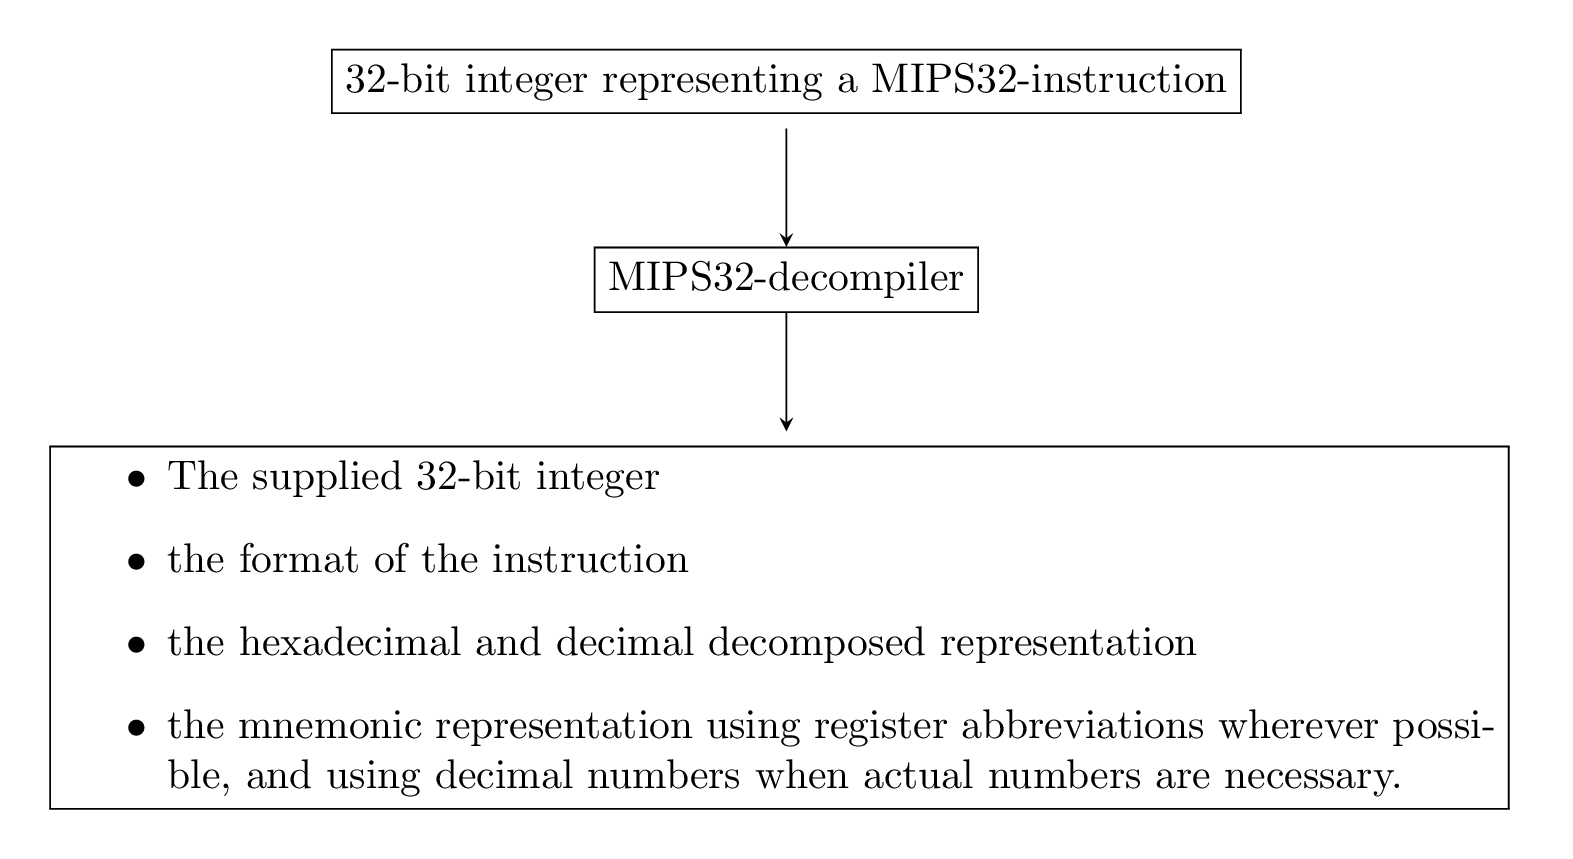
\includegraphics[width=0.9\textwidth]{figures/mips32-decompiler.png}
  \caption{Input and output of the decompiler}
  \label{fig:mips32-decompiler}
\end{figure}



\subsection{Terminology}

% TODO: cite
According to Aho et al.  a \emph{compiler} is a program that
can read a program in one language --- the \emph{source} language --
and translates it into an equivalent program in another language --
the \emph{target} language; see Fig. \ref{fig:compiler}.

\begin{figure}[H]
  \centering
  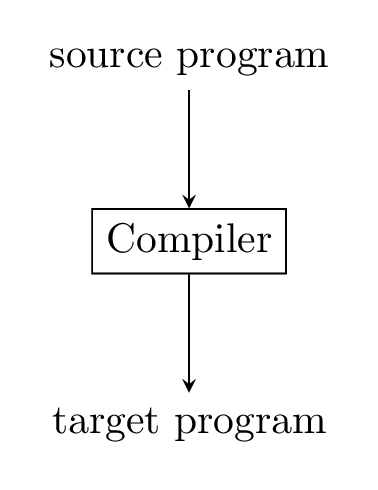
\includegraphics[width=0.3\textwidth]{figures/compiler.png}
  \caption{A compiler}
  \label{fig:compiler}
\end{figure}

Conversely, a \emph{decompiler} is also a that performs the reverse
operation of a compiler. It too, is a compiler. Commonly one views a
compiler as a translator from a high-level human-readable source
language into a low-level machine-readable language, similarly a
decompiler translates in the opposite direction; see
Fig. \ref{fig:decompiler}. 

The two exhibit a chiral relation to one another, i. e. that they are
mirrored images of each other in terms of functionality, but they are
not themselves identical.

\begin{figure}[H]
  \centering
  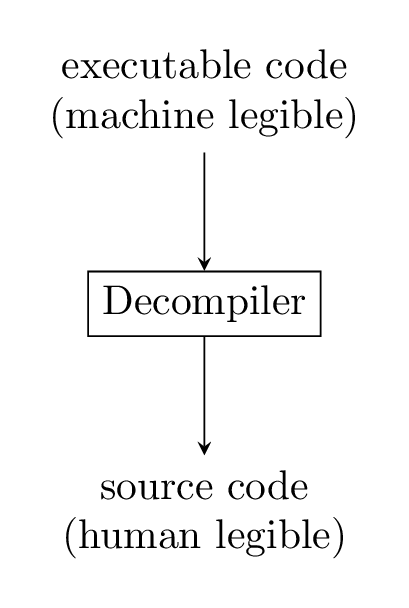
\includegraphics[width=0.3\textwidth]{figures/decompiler.png}
  \caption{A decompiler}
  \label{fig:decompiler}
\end{figure}

In this assignment the decompiler must be able to translate from the
machine-readable language of 32-bit numbers representing MIPS32
instructions to the human-readable target language described in the
introduction.

The constituent parts of the decompilers output will
be described further in section.~\ref{section:mul-example}.

Specifically,

\begin{itemize}
  \item Format.
  \item Opcode.
  \item Decomposed representation.
  \item Mnemonic representation.
\end{itemize}

will be covered. We will augment this list later on.

\subsubsection{Example: Decomposing \texttt{mul}}\label{section:mul-example}

Consider the 32-bit number \texttt{0x71014802}. It is \emph{decomposed}
into fields of varying lengths depending on the \emph{format} of the
instruction.

For all numbers in the MIPS32 instruction set the leftmost six bits
always represent the opcode for the instruction. The opcode alone is
not always sufficient to identify the particular instruction,
\emph{but} it is always sufficient to identify the format of the
instruction.

The leftmost six bits of \texttt{0x71014802} is \texttt{0x1c}. It is
\emph{known} that this number corresponds to an instruction in the
R-format. The format specifies into which fields the remaining bits
decompose into. In Fig. \ref{fig:r-decomposed} each field's size in
bits is the small number below the field.

\begin{figure}[H]
  \centering
  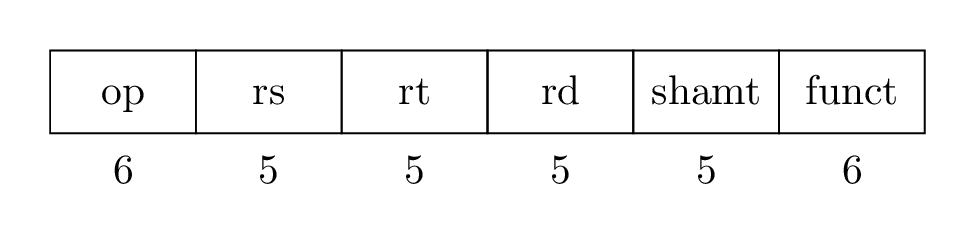
\includegraphics[width=0.9\textwidth]{figures/r-decomposed.png}
  \caption{The fields of an R-type instruction}
  \label{fig:r-decomposed}
\end{figure}

As alluded to previously, all instructions may not be discerned by
their opcode alone. This holds for all R-type instructions.

Decomposing \texttt{0x71014802} into the fields shown in
Fig. \ref{fig:r-decomposed} yields \texttt{rs=8}, \texttt{rt=1},
\texttt{rd=9}, \texttt{shamt=0}, and \texttt{funct=2}. The
\emph{decomposed representation} of this instruction in hexadecimal
form is thus \texttt{[0x1c 8 1 9 0 2]}.\footnote{The corresponding
\emph{decimal representation} is \texttt{[28 8 1 9 0 2]}}

To identify the particular instruction represented by
\texttt{0x71014802} the \texttt{funct} field must be
consulted. Pairing the opcode, \texttt{0x1c} and the value in the
\texttt{funct} field uniquely identifies the instruction a
\texttt{mul} instruction; see Fig. \ref{fig:mul-decomposed}

\begin{figure}[H]
  \centering
  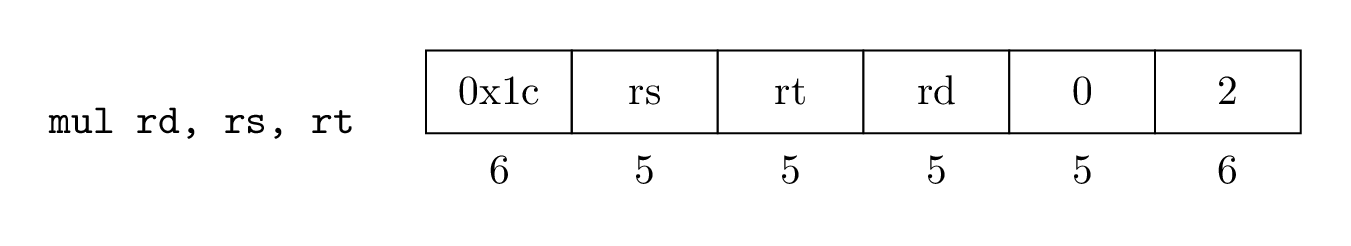
\includegraphics[width=0.9\textwidth]{figures/mul-decomposed.png}
  \caption{Decomposition and mnemonic representation of \texttt{mul}}
  \label{fig:mul-decomposed}
\end{figure}

From Fig. \ref{fig:r-decomposed} the registers \texttt{rs},
\texttt{rt} and \texttt{rd} were determined to have the addresses 8,
1, and 9, respectively. In MIPS registers are named, following the
convention shown in Table. \ref{table:mips-register-naming-convention}

\begin{table}[H]
\centering
\caption{MIPS register naming convention}
\begin{tabular}{ll}
\toprule
Nickname & Register Number \\
\midrule
\$zero      & 0            \\
\$at        & 1            \\
\$v0 - \$v1 & 2 - 3        \\
\$a0 - \$a3 & 4 - 7        \\
\$t0 - \$t7 & 8 - 15       \\
\$s0 - \$s7 & 16 - 23      \\
\$t8 - \$t9 & 24 - 25      \\
\$k0 - \$k1 & 26 - 27      \\
\$gp        & 28           \\
\$sp        & 29           \\
\$fp        & 30           \\
\$rd        & 31           \\
\bottomrule
\end{tabular}
\label{table:mips-register-naming-convention}
\end{table}

Replacing the numerical values of \texttt{rs}, \texttt{rt} and
\texttt{rd}, with their named counterparts yields the \emph{mnemonic
representation} of the instruction to be

\begin{center}
  \texttt{mul \$t1, \$t0, \$at}
\end{center}

\section{Problem statement}\label{section:problem-statement}

In this assignment the core functionality which is exposed is
\emph{parsing} such a 32-bit number representing an instruction from
the MIPS32-instruction set and outputting other representations of the
same instruction, as well as some additional information regarding the
very same instruction, see Fig. \ref{fig:mips32-decompiler}.

\begin{figure}[H]
  \centering
  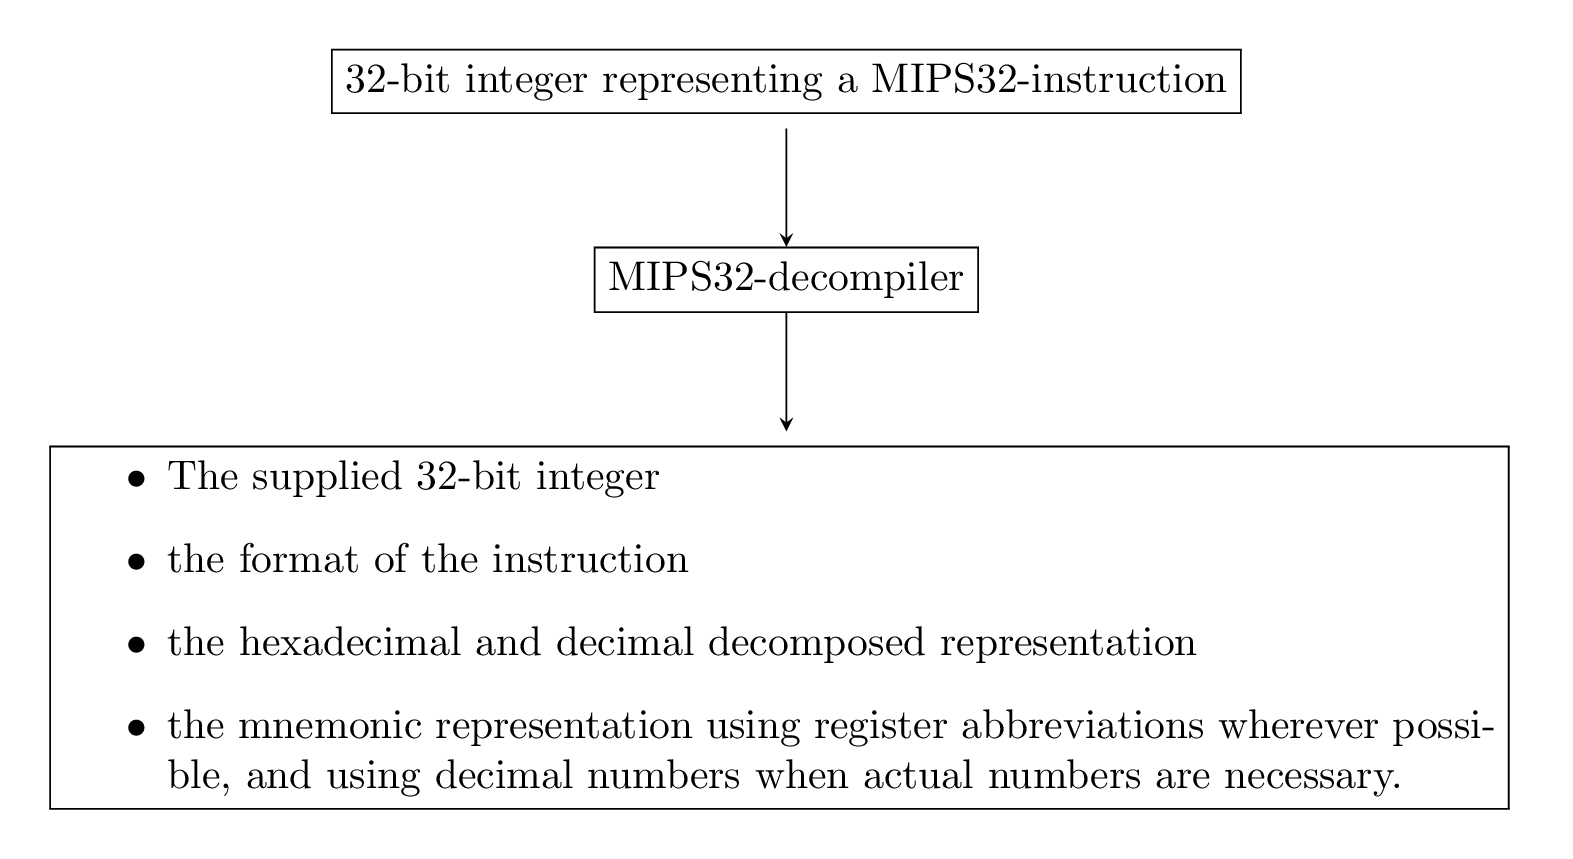
\includegraphics[width=0.9\textwidth]{figures/mips32-decompiler.png}
  \caption{Input and output of the decompiler}
  \label{fig:mips32-decompiler}
\end{figure}

Therefore, we need to be able to identify the appropriate format (from
which we can infer the decomposition), the identity of the particular
instruction (so that we can get its name) and also interpret the
constituent bitfields of the instruction so that we output a mnemonic
representation of the instruction.

In the previous section we established the terminology we will use
throughout the document. This terminology will also be used to
decompose our system that solves the problem at hand, viz. that
we will model our solution according to the problem domain.

Specifically, we will create a system such that when we take in a
32-bit integer representing a valid or semi-valid MIPS32-instruction
then we can construct an object instance named \mij{Instruction} that
knows, or can retrieve information about,\footnote{Using its
collaborators}

\begin{table}
\begin{itemize}
\item Its numerical representation
\item Its own format
\item Its own decomposed representation presented in both:
\subitem Hexadecimal form
\subitem Decimal form
\item Its own mnemonic representation
\end{itemize}
\caption{\mij{Instruction} operations/fields}
\label{table:instruction-operations}
\end{table}

The \mij{Instruction} class is an abstraction providing an
encapsulation around the aforementioned points. Ultimately, the system
will be divided into the self-explanatory constituents

\begin{itemize}
\item \formatm: R, I, J
\item \opcodem: An abstraction around the numerical opcode.
\item \formatm: Can for a given \opcodem return the associated format.
\item \decomposedm: Can decompose a 32-bit number into varying lengths.
\item \registerm: Associates a number with the register name, 
      see Table.~\ref{table:mips-register-naming-convention}
\end{itemize}

The \emph{core} issues to address is that of identifying the
instruction, validating the values of the bitfields of the
instruction, and outputting it according to some \emph{pattern}.

We will now address these issues in more detail, and create a running
tally of functionality that we would like to express within our
system. Afterwards we will define a fascimilie of a domain-specific
language (DSL) that will encode the items we touch upon here.

\subsection{Identifying the instruction}\label{section:identification}

Recall from our earlier example where we decompiled a \tt{mul}
instruction that the \opcode is always sufficient to identify
the format of the instruction it is not always sufficent to
identify an instruction uniquely.

We find that all J-type instructions and for some, but not all, I-type
instructions the \opcode will suffice. Specifically, those I-type
instructions which cannot be identified by their opcode alone is the
branch instructions and immediate trap operations.

For the opcodes \tt{op=0x00}, and \tt{op=0x1c} it is necessary to
consult a second field in order to identify the instruction
completely, namely the \tt{funct} field. For instructions with the
opcode \tt{0x01} the \tt{rt} field must instead be consulted.

Therefore, we would like to compose a system that may

\begin{itemize}
\item Get the six left-most bits from a 32-bit integer, i.e. the numerical opcode.
\item Infer the Format from the opcode.
\item When necessary consult additional bitfields in the 32-bit integer to
      determine the particular instruction.
\end{itemize}

\subsection{Validating the non-identifying bitfields}\label{section:validation}

Consider the 32-bit integer \tt{0x00012122}. This number represents an
instance of the \tt{sub} instruction. It is identified by
having its opcode set to \tt{0x00} and its funct field to \tt{0x22}.
\emph{But}, it is not \emph{valid} if its shamt field is not also set to 0.

This validation step needs to be incorporated somehow. It would be
naive to consider this an additional consultation of a bitfield to
determine identity, since we could not distinguish between whether or
not the correct instruction has been identified or if there is a
problem in the validation.

Hence, our system should be able to (once the particular instruction
has been identified) validate the instruction.

\subsection{Patternizing output}\label{section:patternizing}

We have not addressed this before but the mnemonic representation of
instructions in the MIPS32 instruction set has a tendency to follow a
certain pattern, and these patterns are dependent upon the format of
the particular instruction.

For an example, the instructions

\begin{verbatim}
add, addu, sub, mul, and, or, nor, xor, movn, movz
\end{verbatim}

\newcommand{\pattern}[1]{\emph{$\langle$#1$\rangle$}}
among possibly others, have the common pattern \pattern{iname, rd, rs,
rt} with \emph{iname} being the name of the instruction.

Other common patterns include 

\begin{itemize}
\item \pattern{iname rd, rs}
\item \pattern{iname rd, rt, rs}
\item \pattern{iname, rd, rt, shamt}
\end{itemize}

for R-format instructions and

\begin{itemize}
\item \pattern{iname, rt, rs, imm}
\item \pattern{iname rt, imm}
\item \pattern{iname, rt, rs(addr)}
\end{itemize}

for I-format instructions.

Being a RISC architecture we would expect these patterns to favor
regularity, and that maybe the above set would suffice but there
are in fact numerous others.

As such we will want to, for each instruction, associate it with its
output pattern.

\section{Domain-specific language}

In the previous section.~\ref{section:problem-statement} we described
the \emph{core} issues that our solution needs to address. 

Summarizingly, we found that we want to be able to

\begin{itemize}
\item Get the six left-most bits from a 32-bit integer,
  i.e. the numerical opcode.
\item Infer the Format of the instruction from the opcode.
\item When necessary consult additional bitfields in the 32-bit integer to
      determine the particular instruction.
\item Validate other bitfields when necessary.
\item Convert the numerical representation into a mnemonic representation.
\end{itemize}

The first two items are trivial, the first is the result of a
bit-shift operation and as alluded to previously the Format is always
inferrable from the Opcode, which means that we can either let each
opcode know its associated format or similarily associate formats
with sets of opcodes elsewhere. The specific approach will be covered
later, as will the reason it was chosen.

The subset of the MIPS32-instruction set that we have
implemented,\footnote{Floating point operations and a few others have
  been omitted.} is made up of a large number of operations so we would
like to design our system in such a manner that all of this
\emph{knowledge} pertaining to a particular instruction, viz. how to
validate it and represent it, be stored in a single place.

We want to express this as succinctly as possible, to make it as
legible as possible in one place all the defining characteristics
of an instruction.

Regardless of the instruction type we can express an instruction
as a tuple,

\begin{equation*}
(\langle \textit{identifying characteristics} \rangle, \langle
  \textit{validation requirements} \rangle, \langle \textit{mnemonic
    representation} \rangle)
\end{equation*}





\end{document}
